% ===========================================================================
% Benchmarking — DDS-SLAM / SGS-SLAM / SemanticSuPer on the 5-snippet CRCD bench
% Grounded in the 2026-07-02 results drop (Benchmarking-20260702T131352Z):
%   DDS-SLAM Bench/<snip>_base_s0/{sim3_metrics,render_eval,depth_l1}.txt
%   SGS-SLAM_CRCD_bench5/<snip>/{i.jpg,i_gt.png}  (scored with the same PSNR/SSIM
%     implementation as Addons/eval/eval_rendering.py + LPIPS-alex)
%   SemanticSuperResults/ss_crcd_<snip>/events.out.tfevents (internal telemetry)
% Figures: pub_figures_20260702_benchmark/{dds_trajectories,qualitative,semsup,bars}
% ===========================================================================

\section{Benchmarking on the CRCD Five-Snippet Benchmark}
\label{sec:benchmarking}

All methods are evaluated on the same five rectified CRCD snippets
(C1\_001, C2\_001, C3\_001, E3\_005, G3\_001; 265--1987 frames each), spanning
four patients, camera-still and camera-moving regimes, and tool-quiet through
tool-dominated scenes. Each method consumes the same rectified RGB stream; depth
supervision, where a method requires it, is the same stereo-anchored MoGe-2 depth.
Metrics follow Section~\ref{sec:eval_metrics}. The three systems compared here
occupy deliberately different points in the design space: DDS-SLAM (the base of
this work) is a neural-SDF SLAM that jointly tracks and reconstructs; SGS-SLAM is
a semantic 3D-Gaussian-splatting SLAM; SemanticSuPer is a surfel-based deformable
scene tracker rather than a camera-SLAM system, and is evaluated accordingly.

% ---------------------------------------------------------------------------
\subsection{DDS-SLAM (base configuration)}
\label{sec:bench_dds}

Table~\ref{tab:bench_dds} reports the full battery for the base
configuration (single seed; the C3\_001 run had not completed at the time of
writing and is reported as pending). Three observations structure the analysis:

\begin{table}[t]
\centering
\caption{DDS-SLAM (base) on the CRCD benchmark. Sim(3) ATE in mm; path ratio and
aligned dominant-axis $|r|$ per Section~\ref{sec:eval_metrics}; Depth-$L_1$ is the
input-vs-output self-consistency in mm. C3\_001 pending.}
\label{tab:bench_dds}
\small
\begin{tabular}{lrrrrrrrr}
\toprule
Snippet & $N$ & ATE$_{\mathrm{RMSE}}$ & path ratio & $|r|_{\mathrm{dom}}$ &
PSNR$\uparrow$ & SSIM$\uparrow$ & LPIPS$\downarrow$ & D-$L_1$ \\
\midrule
C1\_001 &  360 & 2.64 &  8.11 & 0.943 & 25.91 & 0.804 & 0.448 &  7.78 \\
C2\_001 &  730 & 6.78 &  8.66 & 0.627 & 22.57 & 0.728 & 0.552 &  8.72 \\
C3\_001 & 1527 & \multicolumn{7}{c}{\emph{pending (run incomplete at time of writing)}} \\
E3\_005 &  265 & 5.31 &  2.62 & 0.480 & 24.93 & 0.801 & 0.483 & 15.44 \\
G3\_001 & 1987 & 4.12 & 18.25 & 0.367 & 29.68 & 0.904 & 0.317 & 10.00 \\
\midrule
mean (4) & --- & 4.71 & 9.41 & 0.604 & 25.77 & 0.809 & 0.450 & 10.49 \\
\bottomrule
\end{tabular}
\end{table}

\paragraph{Tracking is accurate in shape but over-travels.}
Sim(3) ATE sits at 2.6--6.8\,mm across snippets --- small in absolute terms ---
and on C1\_001 the aligned dominant-axis correlation of $0.94$ shows the
trajectory genuinely follows the camera's path. But the path ratios (8.1, 8.7,
18.2 on the low-motion snippets) expose the characteristic disease: the estimate
accumulates many times the true path length. Figure~\ref{fig:bench_traj}
makes this visible --- the ground-truth arc is smooth while the estimate
oscillates around it frame-to-frame. Because CRCD camera motion is sub-SNR
(Section~\ref{sec:eval_metrics}), this jitter costs little ATE, which is
precisely why the path ratio and correlation are mandatory companions to it.
G3\_001 is the extreme case: 1987 frames of near-still camera yield the best
ATE (4.1\,mm) alongside the worst path ratio (18.3) and correlation (0.37) ---
a compact but noisy estimate, not a tracked one.

\paragraph{Rendering tracks scene difficulty.}
PSNR spans 22.6--29.7 across snippets, best on the visually static G3\_001
and worst on C2\_001, whose large gallbladder manipulation both deforms the
scene and drags the (rigid) map behind it. E3\_005's elevated Depth-$L_1$
(15.4\,mm vs.\ 7.8--10.0 elsewhere) reflects the same effect geometrically:
persistent tool--tissue interaction that a rigid SDF cannot absorb.

\begin{figure}[t]
\centering
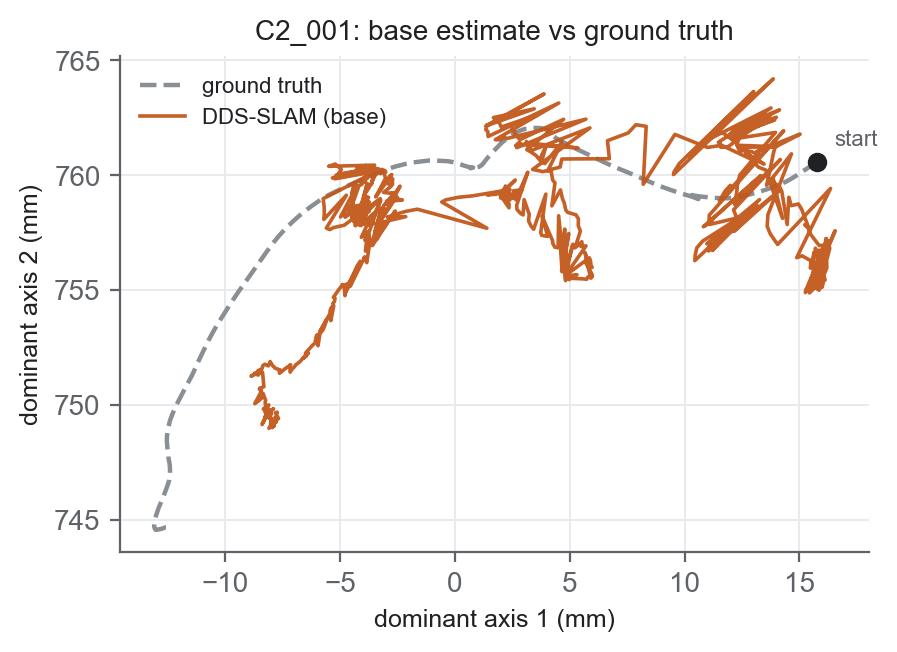
\includegraphics[width=0.49\linewidth]{figures/C2_001_traj_est_vs_gt.png}
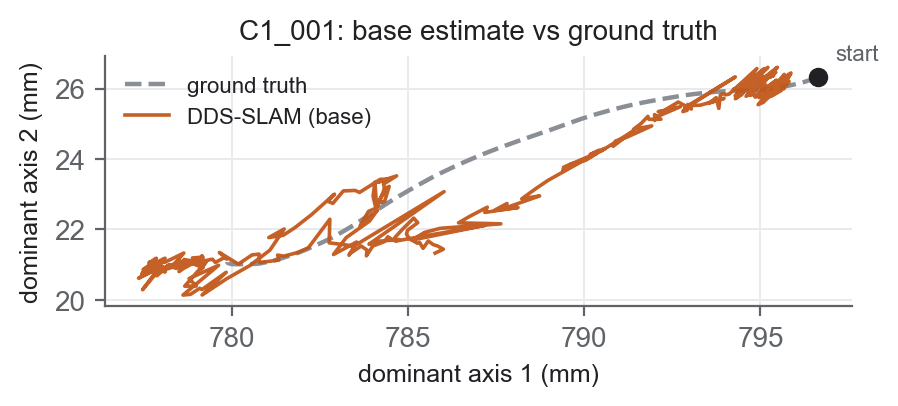
\includegraphics[width=0.49\linewidth]{figures/C1_001_traj_est_vs_gt.png}
\caption{DDS-SLAM (base) estimated trajectory (blue, Sim(3)-aligned) against
ground truth (dashed grey) on C2\_001 (left) and C1\_001 (right). The estimate
follows the true path's shape --- the aligned correlation on C1\_001 is $0.94$
--- but oscillates around it, accumulating $\sim$8$\times$ the true path length:
the over-travel signature that motivates the path-ratio metric and the tracking
contributions of this thesis.}
\label{fig:bench_traj}
\end{figure}

% ---------------------------------------------------------------------------
\subsection{SGS-SLAM}
\label{sec:bench_sgs}

SGS-SLAM \cite{sgsslam} represents the 3D-Gaussian-splatting family: an explicit
anisotropic-Gaussian map optimised per keyframe, with semantic channels. It was
onboarded onto the identical five snippets (same rectified RGB, same depth, its
segmentation head trained on CRCD classes). SGS-SLAM renders every fifth frame
(its keyframe set); rendering metrics in Table~\ref{tab:bench_sgs} are computed
over those rendered keyframes against the corresponding input frames, with the
same PSNR/SSIM implementation and LPIPS network used for DDS-SLAM. It does not
export a comparable camera trajectory in this configuration, so the comparison
is on the mapping half.

\begin{table}[t]
\centering
\caption{SGS-SLAM rendering quality over its rendered keyframes ($n$ per snippet),
scored identically to DDS-SLAM. DDS-SLAM values repeated for comparison
(its metrics cover every frame).}
\label{tab:bench_sgs}
\small
\begin{tabular}{l rrrr c rrr}
\toprule
& \multicolumn{4}{c}{SGS-SLAM} & & \multicolumn{3}{c}{DDS-SLAM (base)} \\
\cmidrule{2-5} \cmidrule{7-9}
Snippet & $n$ & PSNR$\uparrow$ & SSIM$\uparrow$ & LPIPS$\downarrow$ & &
PSNR$\uparrow$ & SSIM$\uparrow$ & LPIPS$\downarrow$ \\
\midrule
C1\_001 &  73 & 22.45 & 0.803 & 0.315 & & 25.91 & 0.804 & 0.448 \\
C2\_001 & 147 & 17.52 & 0.701 & 0.504 & & 22.57 & 0.728 & 0.552 \\
C3\_001 & 306 & 18.78 & 0.798 & 0.508 & & \multicolumn{3}{c}{\emph{pending}} \\
E3\_005 &  54 & 19.15 & 0.780 & 0.397 & & 24.93 & 0.801 & 0.483 \\
G3\_001 & 398 & 18.40 & 0.846 & 0.447 & & 29.68 & 0.904 & 0.317 \\
\bottomrule
\end{tabular}
\end{table}

The pattern is consistent and diagnostic: DDS-SLAM wins PSNR on every
comparable snippet, by margins from $+3.4$\,dB (C1\_001) to $+11.3$\,dB
(G3\_001), while SGS-SLAM wins LPIPS on three of the four (0.315 vs.\ 0.448 on
C1\_001; similarly C2\_001, E3\_005). These are not contradictory --- they are
the two regimes the metric triplet is designed to separate
(Section~\ref{sec:eval_render}). The neural-SDF render is pixel-accurate on
average but soft; the Gaussian render is sharper (better perceptual similarity)
but pays in exact pixel fidelity wherever splats misalign, and it degrades
sharply under the heavy deformation of C2\_001 (17.5\,dB), where a
static explicit map ghosts the moving gallbladder. The exception proves the
rule: on G3\_001 --- long, visually static, deformation-light --- the SDF map
converges far enough that DDS-SLAM takes \emph{both} PSNR (29.7 vs.\ 18.4) and
LPIPS (0.317 vs.\ 0.447); given sufficient optimisation of an undisturbed
scene, the implicit map's advantage becomes unconditional.
Figure~\ref{fig:bench_qual} shows the corresponding qualitative comparison,
and Figure~\ref{fig:bench_bars} the per-snippet bar summary.

\begin{figure}[t]
\centering
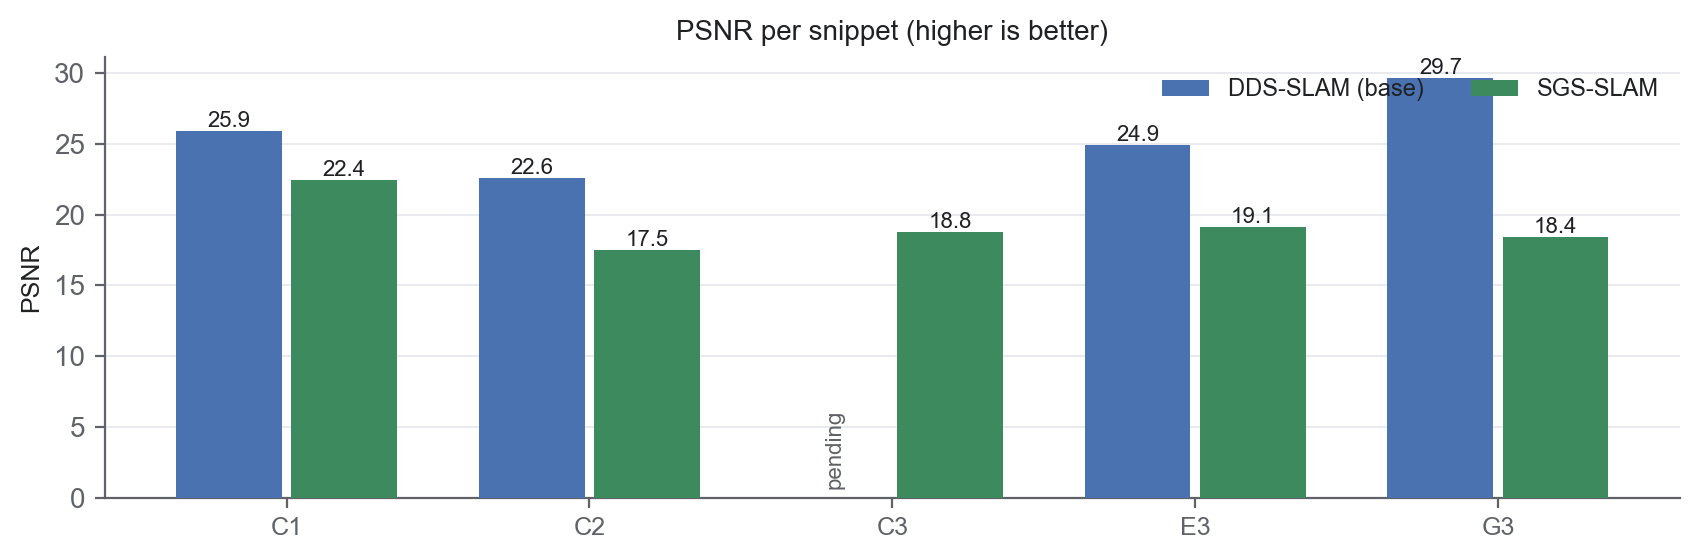
\includegraphics[width=0.85\linewidth]{figures/bench_psnr.png}\\[2pt]
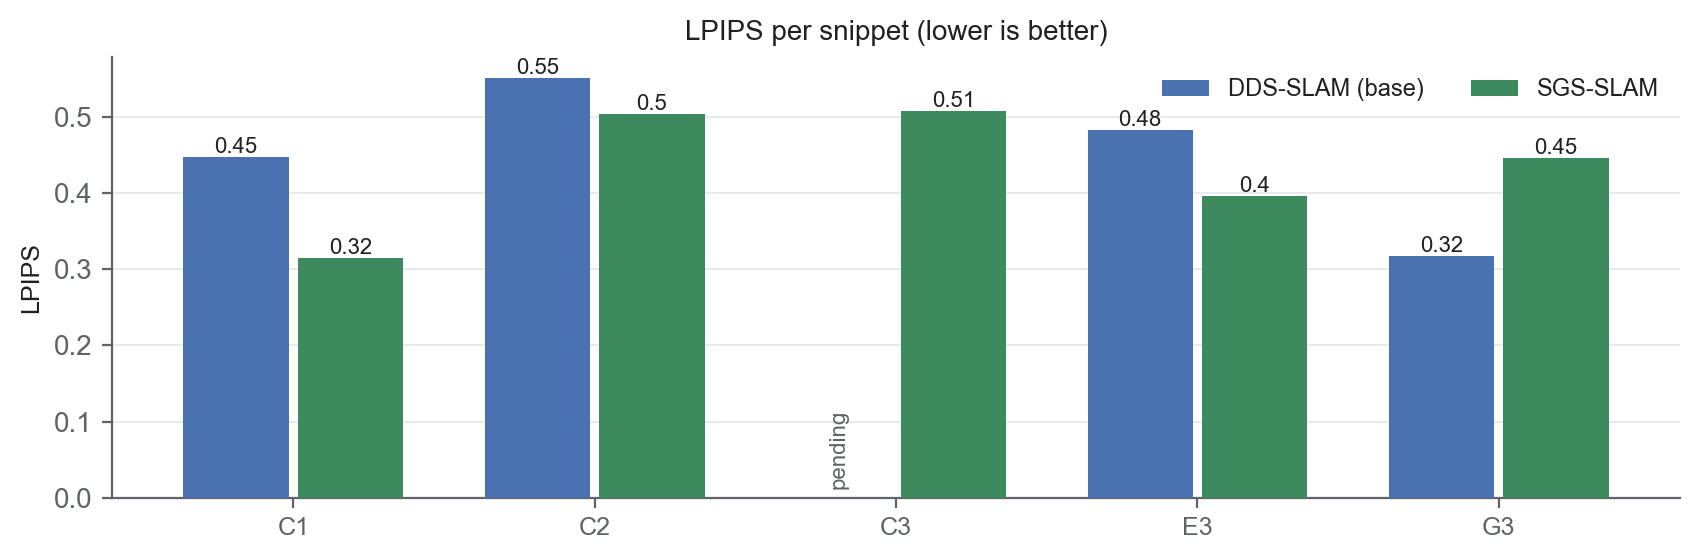
\includegraphics[width=0.85\linewidth]{figures/bench_lpips.png}
\caption{Per-snippet rendering comparison, DDS-SLAM (blue) vs.\ SGS-SLAM
(green): PSNR (top, higher is better) and LPIPS (bottom, lower is better).
DDS-SLAM leads PSNR throughout; SGS-SLAM leads LPIPS except on the static
G3\_001. DDS-SLAM C3\_001 pending.}
\label{fig:bench_bars}
\end{figure}

\begin{figure}[t]
\centering
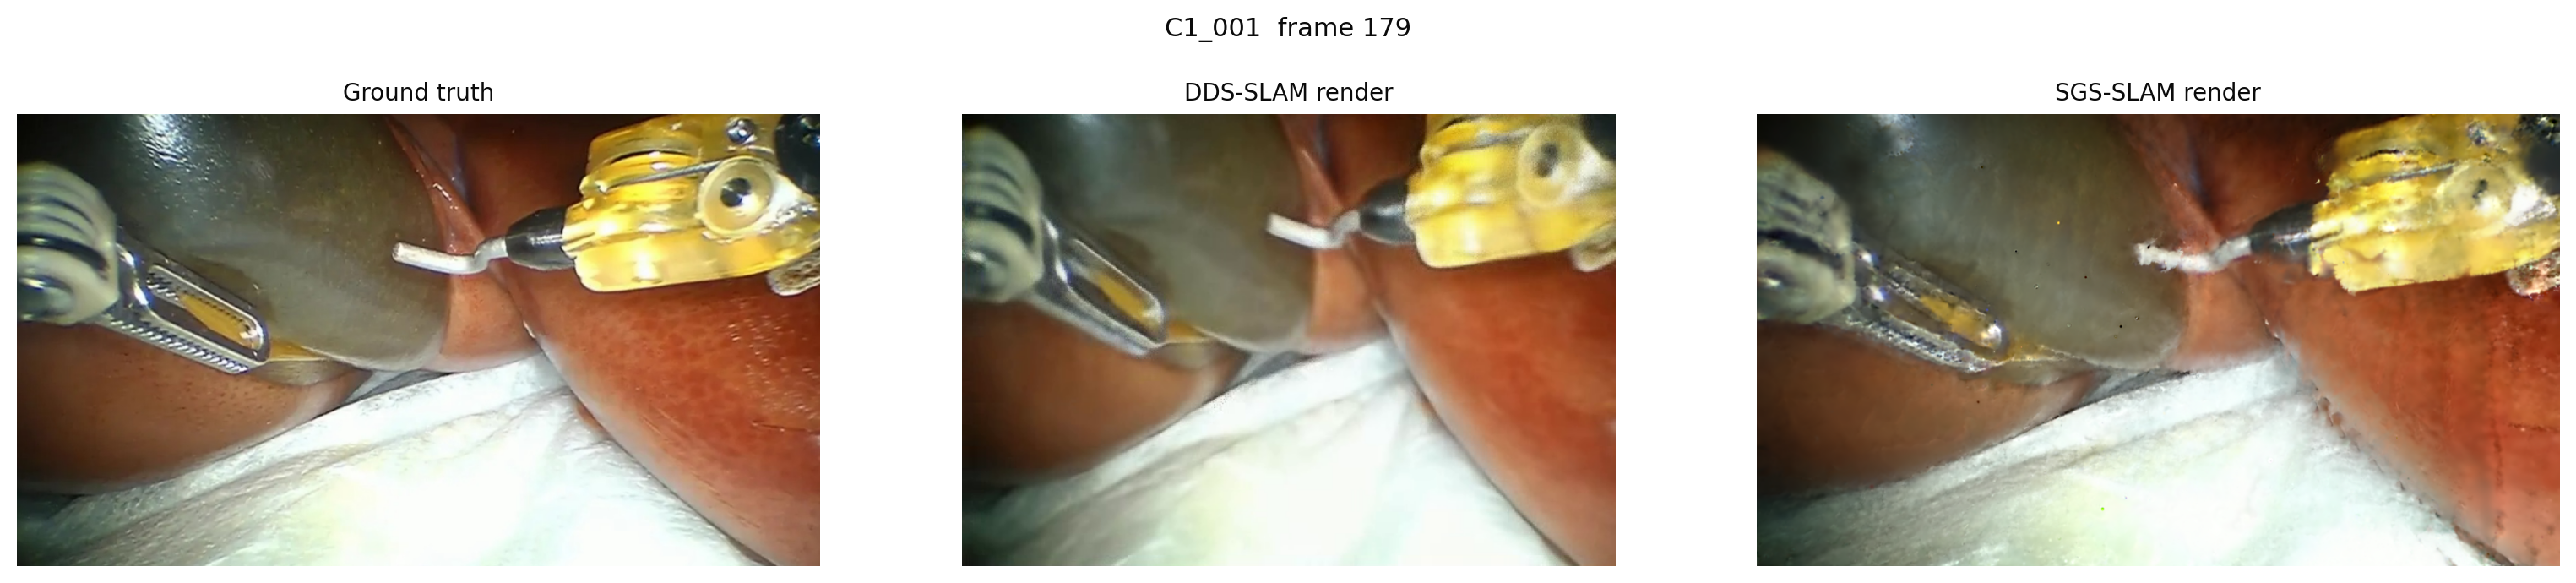
\includegraphics[width=\linewidth]{figures/C1_001_f179_gt_dds_sgs.png}
\caption{Qualitative comparison at C1\_001 frame 179: ground truth (left),
DDS-SLAM render (centre), SGS-SLAM render (right). The DDS-SLAM render is
smoother --- higher PSNR, but soft --- while the SGS-SLAM render preserves more
high-frequency texture (lower LPIPS) at the cost of local splat artefacts.}
\label{fig:bench_qual}
\end{figure}

% ---------------------------------------------------------------------------
\subsection{SemGauss-SLAM}
\label{sec:bench_semgauss}

SemGauss-SLAM \cite{semgauss} is the semantic-feature-field Gaussian
representative. It shares the SplaTAM lineage with SGS-SLAM --- the same
tracking-by-rasterisation, keyframe mapping and densify-and-prune machinery ---
which makes the pair a controlled comparison: the one substantive difference is
that SemGauss-SLAM attaches a 16-dimensional semantic feature to every
Gaussian, rasterises it as an additional feature image, and distils it against
a DINOv2 segmentation head during mapping. It was onboarded onto the identical
five rectified snippets with only per-dataset values changed (intrinsics,
depth scale, class count); every optimisation hyperparameter is the authors'
Replica value verbatim. The segmentation head is our in-domain four-class
DINOv2 head with the benchmark snippet held out of its training, and semantics
run in the authors' default self-supervised mode (no ground-truth masks enter
any loss). Unlike SGS-SLAM's configuration, SemGauss-SLAM exports its full
camera state, so it is scored on \emph{both} halves of the problem: Sim(3) ATE,
path ratio and aligned $|r|_{\mathrm{dom}}$ on its native trajectory, and
every-frame renders under the identical PSNR/SSIM/LPIPS and Depth-$L_1$
pipeline (Table~\ref{tab:bench_semgauss}).

\begin{table}[t]
\centering
\caption{SemGauss-SLAM on the CRCD benchmark, scored identically to DDS-SLAM:
native trajectory under Sim(3) (ATE in mm) and every-frame renders. LPIPS on
three snippets awaits a rescore (scorer library missing on the compute host at
run time; renders retained). G3\_001 exceeds an A100-80GB before half sequence
(see text) and is scored on its first 750 frames against the matching
ground-truth prefix.}
\label{tab:bench_semgauss}
\small
\begin{tabular}{l r rrrr rrrr}
\toprule
Snippet & $N$ & ATE$_{\mathrm{mean}}$ & ATE$_{\mathrm{max}}$ & path ratio &
$|r|_{\mathrm{dom}}$ & PSNR$\uparrow$ & SSIM$\uparrow$ & LPIPS$\downarrow$ & D-$L_1$ \\
\midrule
C1\_001 &  360 & 5.98 & 14.38 &  3.25 & 0.76 & 20.57 & 0.771 & 0.344 & 22.5 \\
C2\_001 &  730 & 7.25 & 21.78 & 13.14 & 0.80 & 16.31 & 0.674 & ---   & 44.2 \\
C3\_001 & 1527 & 8.14 & 25.75 & 23.60 & 0.90 & 17.78 & 0.783 & ---   & 24.6 \\
E3\_005 &  265 & 5.12 & 16.84 &  1.70 & 0.34 & 17.31 & 0.726 & ---   & 50.0 \\
G3\_001 & 750$^{\dagger}$ & \multicolumn{8}{c}{\emph{in progress}} \\
\midrule
mean (4) & --- & 6.62 & 19.69 & 10.42 & 0.70 & 17.99 & 0.739 & --- & 35.3 \\
\bottomrule
\multicolumn{10}{l}{\footnotesize $^{\dagger}$first 750 of 1987 frames
(memory ceiling, see text); evaluated against the corresponding GT prefix.}
\end{tabular}
\end{table}

Against its architectural sibling the pattern is uniform: SemGauss-SLAM renders
1--2\,dB below SGS-SLAM on every shared snippet (20.6 vs.\ 22.5 on C1\_001,
16.3 vs.\ 17.5 on C2\_001, 17.8 vs.\ 18.8 on C3\_001, 17.3 vs.\ 19.2 on
E3\_005) --- the per-Gaussian feature field buys dense distilled semantics and
costs a consistent photometric margin. Its tracking, however, is genuinely
comparable where SGS-SLAM's configuration offers none: Sim(3) ATE of
5--8\,mm with dominant-axis correlations of 0.76--0.90 on the C-snippets,
degrading to $|r|_{\mathrm{dom}}=0.34$ on E3\_005 --- the same sub-SNR
collapse every system shows on that snippet, and the case the path-ratio and
correlation columns exist to expose.

The G3\_001 failure is the section's most instructive result, because it is a
\emph{scaling} property rather than a crash. On an A100-80GB the run exhausted
memory at frame 863 of 1987 with 76.5\,GiB allocated against 76.8 reserved ---
genuine capacity exhaustion, not fragmentation. The driver is not sequence
length but densification rate: SplaTAM-family methods add Gaussians wherever
the current map fails to explain the frame, so the map grows with
newly-revealed surface, and G3\_001's exploratory camera and tool activity
never let it plateau. The checkpoint counts make the mechanism explicit:
C1\_001, C2\_001 and C3\_001 finish with 1.75--1.78\,M Gaussians (C3\_001 over
its full 1527 frames), E3\_005 with 2.77\,M --- while G3\_001 had accumulated
11.0\,M by frame ${\sim}600$, six times C3\_001's final count at a third of
the sequence. SGS-SLAM completed the same snippet on the same GPU: its
Gaussians are roughly $3\times$ lighter, carrying no 16-d feature vector, no
16-channel rasterisation buffers and no corresponding gradients. The authors'
configuration exposes no Gaussian budget --- Replica never needed one --- so
the ceiling is a property of the method, not of our port: the semantic feature
field trades memory scalability for its dense semantics, and an exploratory
endoscopic sequence is precisely the regime that collects the bill. The
main-table entry is therefore the faithful run over the first 750 frames,
evaluated against the matching ground-truth prefix; a pruning-tightened
variant (densification gate 0.5$\rightarrow$0.25, prune threshold
0.005$\rightarrow$0.05, pruning throughout the mapping window) is additionally
run as an explicitly non-faithful ablation to quantify the memory--quality
trade of that feature field, and is reported as a side note rather than a
benchmark row.

% TODO figure once plotted from vram_samples.txt + checkpoint counts:
% \begin{figure}[t]
% \centering
% \includegraphics[width=0.9\linewidth]{figures/semgauss_gaussian_growth.pdf}
% \caption{Gaussian count and VRAM growth, G3\_001 vs.\ C3\_001. C3\_001
% plateaus below 2M Gaussians; G3\_001's exploratory camera never lets
% densification saturate, crossing 11M (${>}$80\,GB) before half sequence.}
% \label{fig:semgauss_growth}
% \end{figure}

% ---------------------------------------------------------------------------
\subsection{SemanticSuPer}
\label{sec:bench_semsup}

SemanticSuPer \cite{semanticsuper} is included as the deformable-reconstruction
representative: a semantic surfel graph with embedded-deformation (ED) nodes,
optimised per frame against depth, photometric and semantic terms. It is not a
camera-SLAM system --- the camera is assumed static while the surfel graph
deforms --- so neither trajectory metrics nor like-for-like render metrics apply;
its shipped output in this benchmark is internal telemetry (per-frame losses,
graph statistics, timing), summarised in Table~\ref{tab:bench_semsup} and
Figure~\ref{fig:bench_semsup}.

\begin{table}[t]
\centering
\caption{SemanticSuPer on the CRCD benchmark --- internal telemetry (no
trajectory or comparable render output is produced in this configuration).
Surfel count is the final frame's; the embedded-deformation graph is fixed at
1197 nodes on every snippet. Render loss is the method's \emph{own} photometric
objective at the final processed frame --- an internal convergence indicator,
not comparable across methods.}
\label{tab:bench_semsup}
\small
\begin{tabular}{l rr r r r}
\toprule
Snippet & frames done & of & surfels ($10^3$) & med.\ time/frame (s) & final render loss \\
\midrule
C1\_001 &  360 &  360 & 159.9 & 2.29 & 0.0111 \\
C2\_001 &   43 &  730 &  27.2 & 1.26 & 0.0082$^{\dagger}$ \\
C3\_001 & 1527 & 1527 &  98.9 & 1.58 & 0.0052 \\
E3\_005 &  265 &  265 & 105.1 & 1.74 & 0.0034 \\
G3\_001 & 1987 & 1987 &  30.8 & 1.18 & 0.0029 \\
\bottomrule
\multicolumn{6}{l}{\footnotesize $^{\dagger}$at the halt frame (43/730), not a
completed-sequence value.}
\end{tabular}
\end{table}

Three facts are relevant to the comparison. First, \emph{it runs}: four of five
snippets processed to completion at 1.2--2.3\,s per frame (median), maintaining
$3\times10^4$--$1.6\times10^5$ surfels and a fixed 1197-node ED graph ---
deformable surgical scenes are within its operating envelope. Second,
\emph{C2\_001 fails early}: processing halts at frame 43 of 730, during the
gallbladder retraction whose large occlusions and topology change break
surfel--frame association --- the same sequence that is the hardest for both
renderers above, and a useful marker of where all three paradigms strain.
Third, the ED-graph formulation \emph{presumes} the deformation--camera split
that this thesis has to estimate: with a moving endoscope, per-frame scene
deformation and camera motion are entangled in exactly the way
Chapter~\ref{sec:tracking_limits} describes, which is why SemanticSuPer's
telemetry is reported here as context rather than as a competing tracking or
rendering result.

\begin{figure}[t]
\centering
\includegraphics[width=\linewidth]{figures/semsup_telemetry.png}
\caption{SemanticSuPer internal telemetry on the five benchmark snippets.
Left: surfel count over each sequence. Right: median per-frame optimisation
time; C2\_001 (aqua) halts at frame 43 of 730 during the gallbladder
retraction.}
\label{fig:bench_semsup}
\end{figure}

% ---------------------------------------------------------------------------
\subsection{PERSEUS}
\label{sec:bench_perseus}

PERSEUS \cite{perseus} is the learned dense-bundle-adjustment representative:
a DROID-SLAM \cite{teed2021droid} derivative in which a recurrent optical-flow
network drives dense per-keyframe bundle adjustment, extended with semantic
segmentation and monocular depth submodules that label the reconstructed point
cloud. It is the only monocular system in the benchmark --- it consumes the
rectified RGB stream and intrinsics alone, with no depth input --- and the
only one whose map exists purely in service of tracking. Its entry is
therefore the mirror image of SGS-SLAM's: tracking-only. It renders nothing,
so PSNR/SSIM/LPIPS do not apply, and it takes no depth in, so the
input-versus-output Depth-$L_1$ self-consistency is undefined; its native
trajectory is up-to-scale, which is precisely the case the Sim(3) protocol
exists for. Onboarding required no method configuration at all: every DROID
hyperparameter is the authors' default, and the only dataset-side inputs are
the calibration file (rectified intrinsics, zero distortion) and a frame
stride of one (the shipped default of three would emit a third of the poses
and break frame-exact pairing with ground truth). Two mechanical repairs to
the published code were necessary and are documented in the runbook: the
released fork ships its trajectory-export path commented out (as published it
cannot emit a trajectory), which we restored from the authors' own
commented-out upstream lines; and the segmentation submodule --- trained on
central-airway anatomy and hard-coded to a circular endoscope mask --- is
bypassed with a null stub. The bypass is provably tracking-identical: the
segmentation mask is stored only for point-cloud labelling and is never
consumed by the motion filter, factor graph or bundle adjustment, so the
tracking numbers are unaffected; the semantic half of PERSEUS is simply
out of domain on colorectal data and is noted as such rather than scored.

\begin{table}[t]
\centering
\caption{PERSEUS on the CRCD benchmark: Sim(3) ATE (mm), path ratio and
aligned $|r|_{\mathrm{dom}}$ on its native monocular trajectory (frame stride
1, all DROID hyperparameters at the authors' defaults). Render and
Depth-$L_1$ columns do not apply (Section~\ref{sec:bench_perseus}).}
\label{tab:bench_perseus}
\small
\begin{tabular}{l r rrrr}
\toprule
Snippet & $N$ & ATE$_{\mathrm{mean}}$ & ATE$_{\mathrm{max}}$ & path ratio &
$|r|_{\mathrm{dom}}$ \\
\midrule
C1\_001 &  360 &  1.97 &  4.64 & 3.31 & 0.97 \\
C2\_001 &  730 &  3.64 & 10.46 & 2.93 & 0.98 \\
C3\_001 & 1527 & 10.69 & 21.90 & 0.96 & 0.48 \\
E3\_005 &  265 &  4.84 & 14.83 & 0.51 & 0.18 \\
G3\_001 & 1987 &  4.87 & 14.63 & 5.03 & 0.52 \\
\midrule
mean (5) & --- & 5.20 & 13.29 & 2.55 & 0.63 \\
\bottomrule
\end{tabular}
\end{table}

The results split cleanly along the benchmark's own fault line. On the
deformation-heavy retraction snippets PERSEUS sets the tracking bar for the
entire table: C1\_001 at 1.97\,mm with $|r|_{\mathrm{dom}}=0.97$ and C2\_001
at 3.64\,mm with $|r|_{\mathrm{dom}}=0.98$ --- the latter on the sequence
that degrades every render-based system, roughly halving the best Gaussian
ATE (SGS-SLAM offers no trajectory; SemGauss-SLAM: 7.25\,mm at path ratio
13.1). Its path ratios are equally diagnostic: 0.5--5$\times$ across all five
snippets, against the 3--24$\times$ of the render-loss trackers --- dense
flow-based bundle adjustment simply does not over-travel, because its
correspondences come from a learned matcher rather than from a photometric
loss chasing noise. On the sub-SNR snippets the failure mode inverts rather
than repeats: E3\_005 collapses to $|r|_{\mathrm{dom}}=0.18$ with a path
ratio of \emph{0.51} --- under-travel, not over-travel --- as DROID's motion
filter gates frames whose optical flow falls below its threshold and the
estimate simply stops moving with the camera. The same regime that makes
photometric trackers wander therefore makes a flow tracker freeze; neither
family observes millimetre-scale motion reliably, which is precisely the
sub-SNR argument of Section~\ref{sec:bench_summary} made from the opposite
direction. Benchmark rows are the segmentation-stubbed arm (provably
tracking-identical, Section above); the faithful segmentation path
additionally cannot load its own released checkpoint.

% ---------------------------------------------------------------------------
\subsection{Cross-method summary}
\label{sec:bench_summary}

No single system dominates. DDS-SLAM is the only one of the three that
\emph{tracks} the camera, and its weakness is behavioural (over-travel on
sub-SNR motion) rather than catastrophic; SGS-SLAM produces the perceptually
sharpest renders but degrades fastest under deformation and offers no
trajectory here; SemanticSuPer handles deformation explicitly but assumes away
the camera problem and fails outright on the heaviest-manipulation snippet.
C2\_001 --- large tissue retraction under camera motion --- is the common
stress case across all three, and is where the contributions of this thesis
(uncertainty-weighted tracking and motion-aware supervision on the SDF
substrate) are aimed.
